\documentclass[english]{article}
\usepackage[T1]{fontenc}
%\usepackage[latin9]{inputenc}
%\usepackage{geometry}
%\geometry{verbose,tmargin=1in,bmargin=1in,lmargin=1in,rmargin=1in}
\usepackage{amsmath}
\usepackage{amssymb}
\usepackage{setspace}
\usepackage[utf8]{inputenc}
\usepackage{graphicx}
\usepackage{float}
\usepackage{adjustbox}
\usepackage{gensymb}
\usepackage{amssymb}
\usepackage{array}
\usepackage{ragged2e}
\usepackage{lipsum}
\onehalfspacing
\usepackage{babel}
\usepackage{tikz}
\usepackage{ctable}
\usepackage{booktabs}
\usepackage{graphicx}
\usepackage{caption}
\usepackage{placeins}
\usepackage{todonotes}
\usepackage{subcaption}
\usepackage[font=footnotesize,labelformat=simple]{subcaption}
\usepackage[T1]{fontenc}
\usepackage{pdflscape}

\begin{document}


\title{Informality and self -employment in the last 20 years}
\maketitle
\begin{itemize}
\item The 2005-2015 decade was characterize by the upswing of the commodity super-cycle.  The 2015-today was started by the downfall of commodity prices, and has remained disappointing in terms of GDP growth. The Good news is that informality decreased in the first decade and didn't seems to have increased in the last decade. 

 Figures on the evolution of informality and self-employment with three bars 2005 2015 and last year [let's see the lac average first and then decide on the final format of the figure]

    \item What is the composition of Labor markets in the average country ( with country by country figures in the appendix for now) LAC pie chart with the following categories: dependent worker contributing to ss, self-employed (a todos b by ss c), non-contributing dependent workers in small firm, non-contributing dependent worker in large firm) [Pie 2005- 2015-Pie Last year]
    \item Informality/self-employment have different set of prevalence across worker characteristics:
    Fig 13. Share of Workers Who Do Not Contribute to Social Security by Selected Characteristics INCLUDE WOMEN, INCLUDE YOUNG Workers Include poor (after we keep this variable in the next round of sedlac), and version with self-employment 
    \item Life-cycle pattern 
    The life-cycle pattern shows that the dependent informal and the self-employed play different role in the informality landscape. Do this by education level as well.
    
    \item Disaggregation of informal employment into self-employed and dependent informal.
    \item Share of informal workers by economic sector (services, commerce, agriculture, manufacturing etc.)
    \item Informality and GDP per Capita
    
    
    \end{itemize}
    \section{Self-employment}
    
    
    
    \begin{itemize}
        \item Self employed can be of different types, with the data from household surveys we can double click on self-employed workers and see what share has college or more, what share has low education and is own account. 
        (Pies)
        \item Share of self employed by income decile ( \cite{herreno_macroeconomic_2023})
        \item What share of self-employed live in a household with a worker contributing to ss (columna por pais para el ultimo año)
        \item Share of self-employed who are informal
        \item Which industries concentrate self-employed workers 
        \item Using matrix data: Share of self-employed who move to formal jobs over time. How long people stay in self-employment.
        \item Self-Employment and GDP
        
    \end{itemize}

\section {What do we know about dependent-informal workers?}    
\begin{itemize}
     \item Share of dependents by type of contract
    \item Dependent informality rate by age over education and gender
    \item Share that works in a small firm  
    \item Compare written vs. verbal contracts against whether they contribute or not.
    \item Using matrix data: Show probability of moving from informal dependent work to formal
    \item Informal dependents and business cycle: Show how dependent informality behaves during expansions vs. recessions.
\end{itemize}

\section{Shares}

\begin{figure}[H]
            \justifying
                \caption{Share of employers of a small firms: owner of a firm with growth potential}  
            \centerline{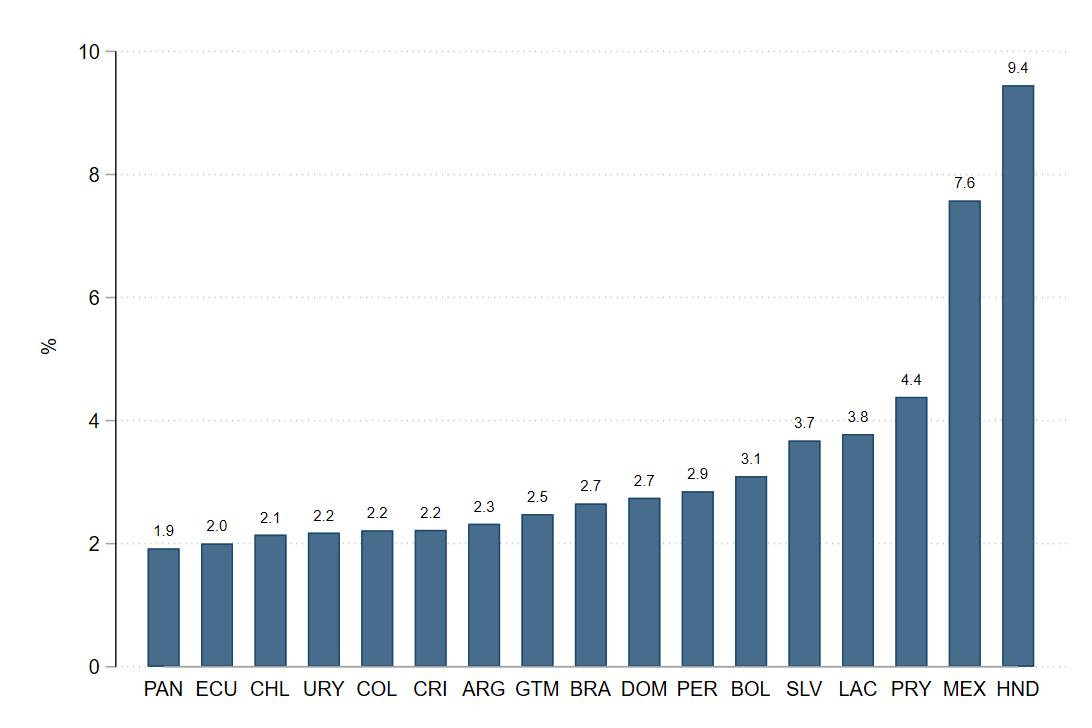
\includegraphics[scale=.3]{latex/figures/Self-employed/employer_growthfirms.png}}
                \label{fig:owner}
                \footnotesize{Source: SEDLAC}
\end{figure}

\begin{figure}[H]
            \justifying
                \caption{Share of self-employed (independents and employers) who work in small firms}  
            \centerline{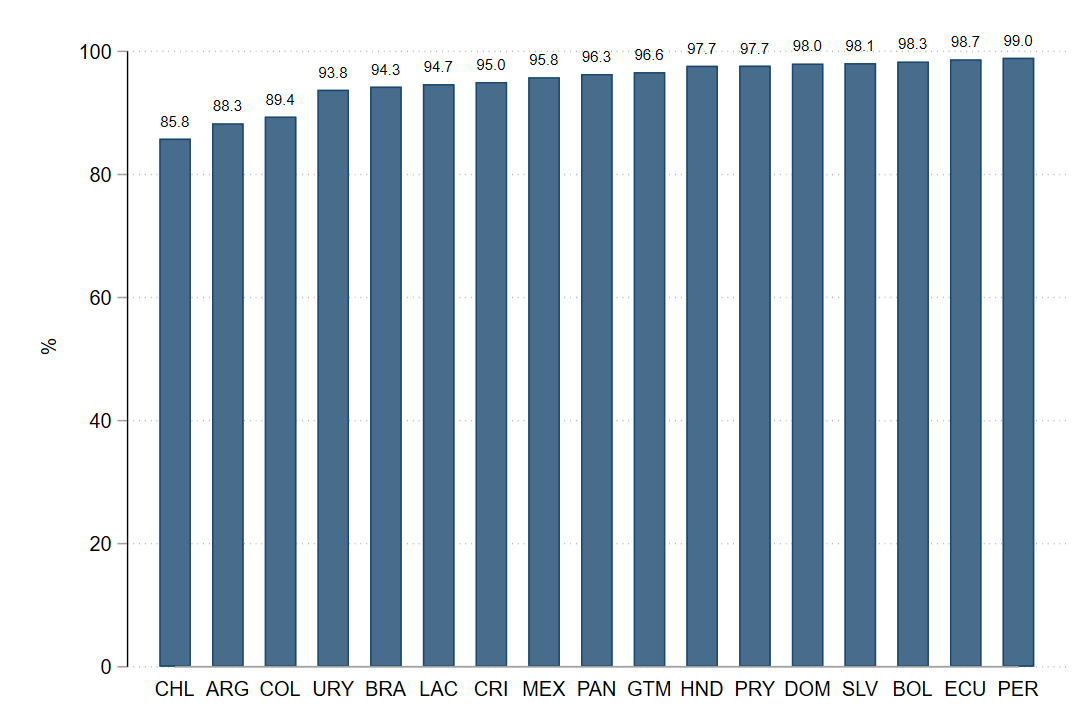
\includegraphics[scale=.3]{latex/figures/Self-employed/selfemployed_small.png}}
                \label{fig:se-small}
                \footnotesize{Source: SEDLAC}
\end{figure}

\begin{figure}[H]
            \justifying
                \caption{Share of self-employed (without employees): independent contractor or own account}  
            \centerline{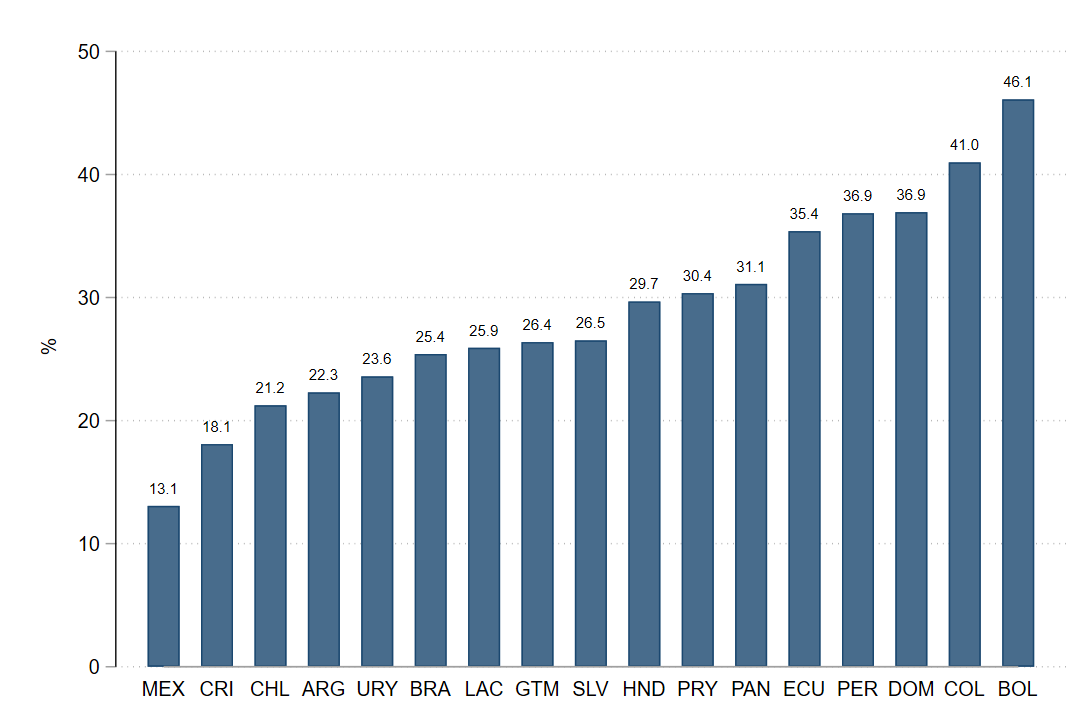
\includegraphics[scale=.3]{latex/figures/Self-employed/independent.png}}
                \label{fig:independent}
                \footnotesize{Source: SEDLAC}
\end{figure}


\section{Contributes to SS}

\begin{figure}[H]
            \justifying
                \caption{Share of employers of small firms who does not contributes to SS}  
            \centerline{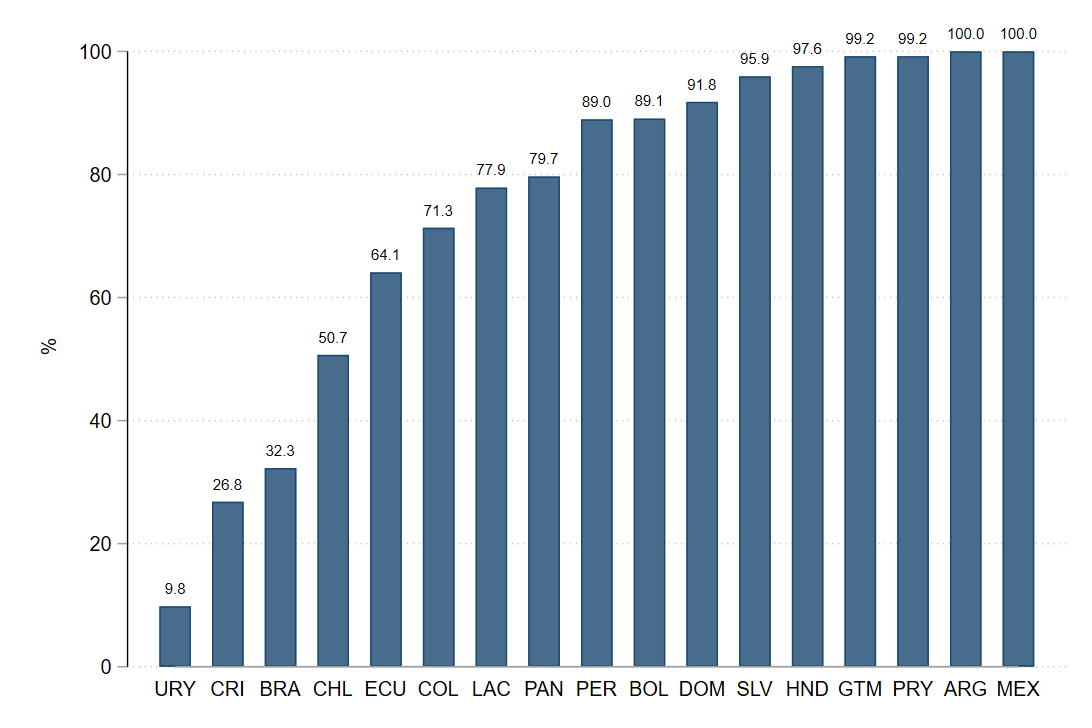
\includegraphics[scale=.3]{latex/figures/Self-employed/i_empgrowthfirm.png}}
                \label{fig:i-employers}
                \footnotesize{Source: SEDLAC}
\end{figure}

\begin{figure}[H]
            \justifying
                \caption{Share of self-employed (independents and employers) who work in small firms and does not contributes to SS}  
            \centerline{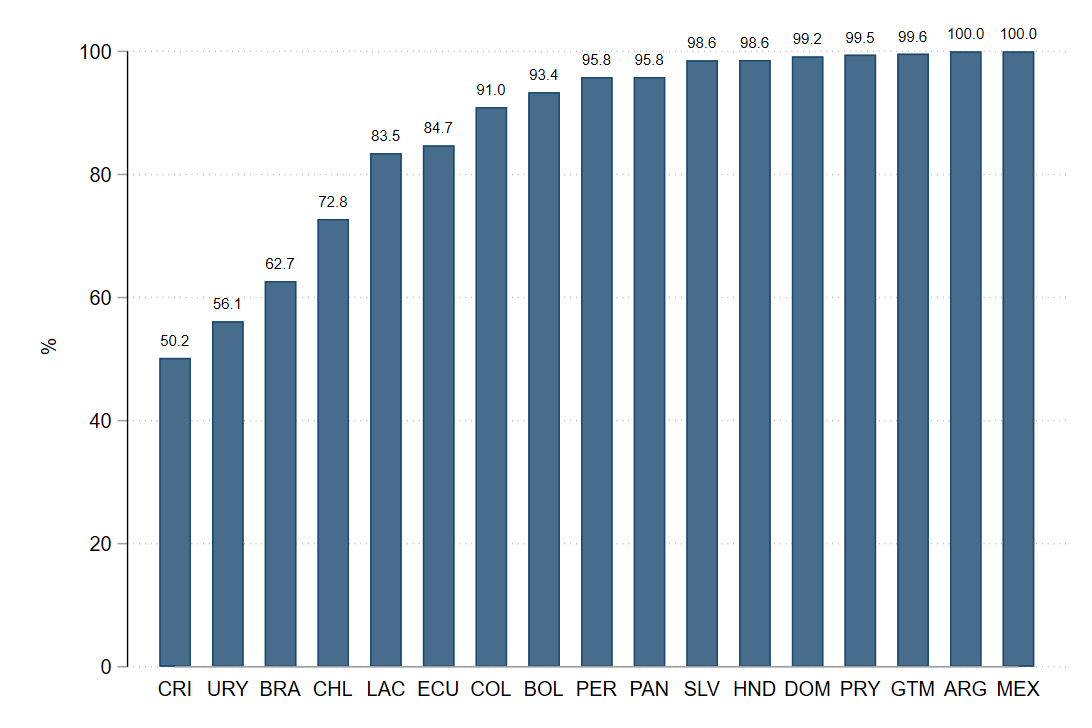
\includegraphics[scale=.3]{latex/figures/Self-employed/i_selfsmall.png}}
                \label{fig:i-se}
                \footnotesize{Source: SEDLAC}
\end{figure}

\begin{figure}[H]
            \justifying
                \caption{Share of self-employed (without employers) who does not contributes to SS: independent contractor}  
            \centerline{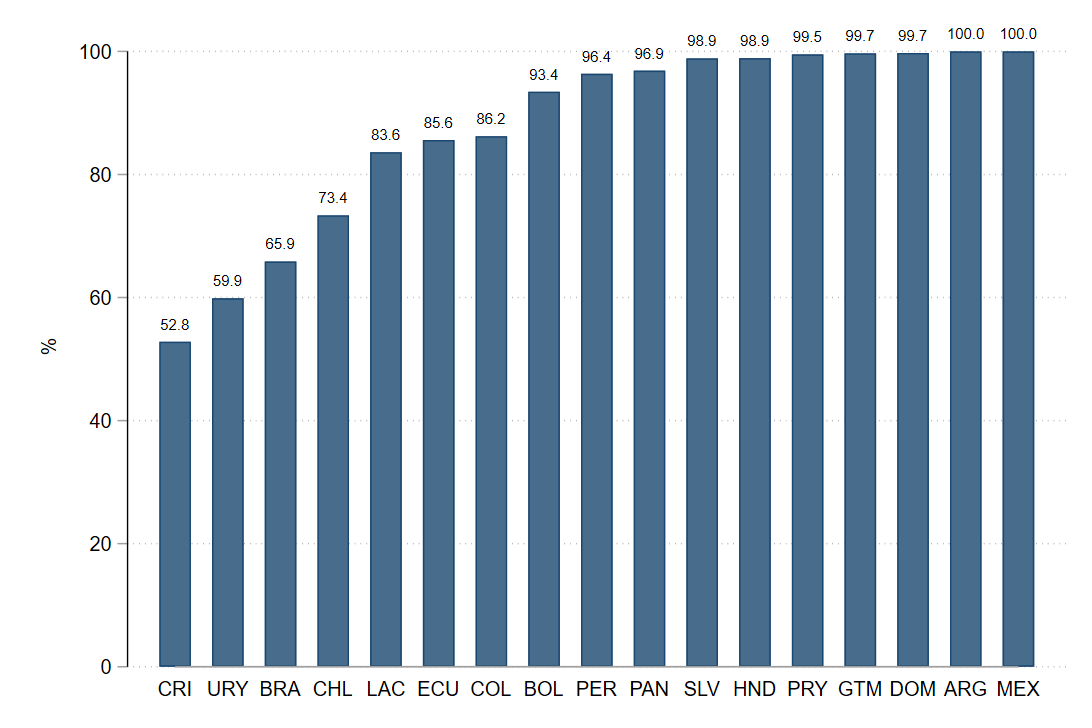
\includegraphics[scale=.3]{latex/figures/Self-employed/i_independent.png}}
                \label{fig:i-independents}
                \footnotesize{Source: SEDLAC}
\end{figure}


\begin{figure}[H]
            \justifying
                \caption{Share of not salaried workers in small firms}  
            \centerline{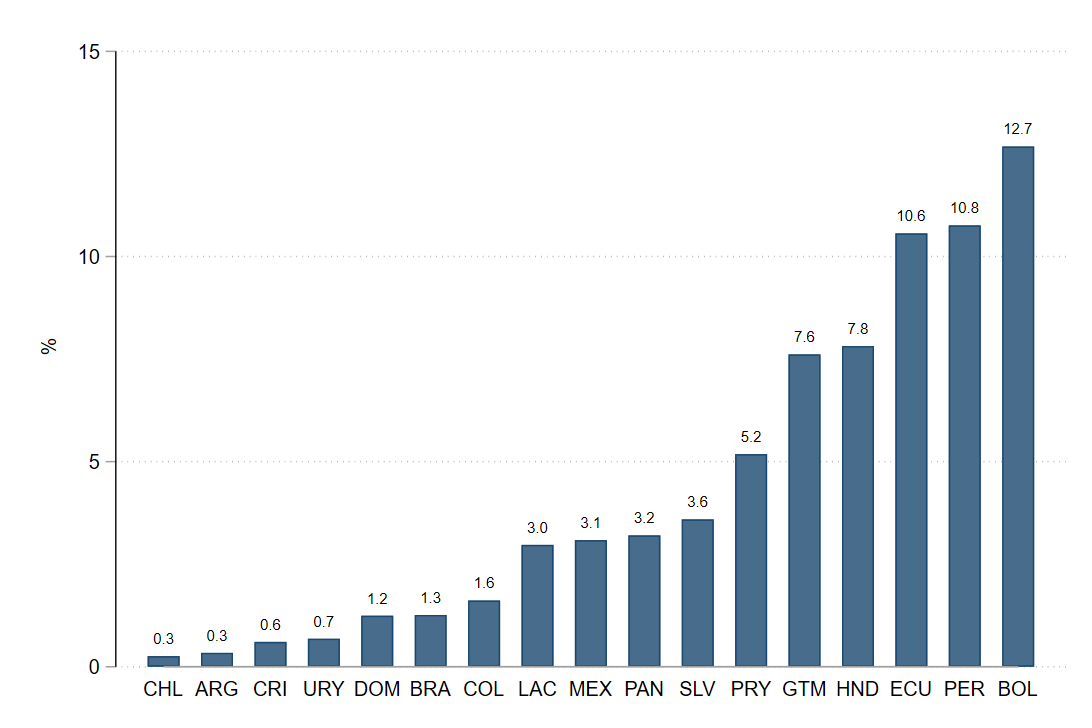
\includegraphics[scale=.3]{latex/figures/Self-employed/notsalaried_small.png}}
                \label{fig:notsalaried}
                \footnotesize{Source: SEDLAC}
\end{figure}

\begin{figure}[H]
            \justifying
                \caption{Share of self-employed in households where at least one person contributes to SS}  
            \centerline{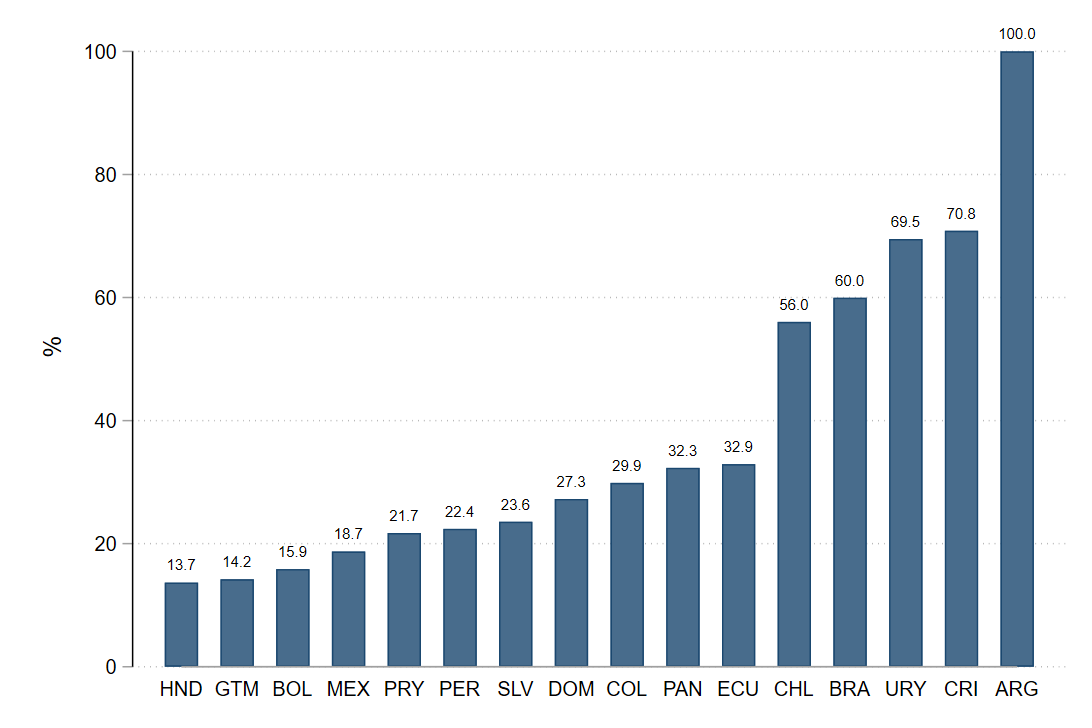
\includegraphics[scale=.3]{latex/figures/Self-employed/se_contribuye_hogar.png}}
                \label{fig:se-one}
                \footnotesize{Source: SEDLAC}
\end{figure}

\begin{figure}[H]
            \justifying
                \caption{Share of self-employed in households with at least two employed people}  
            \centerline{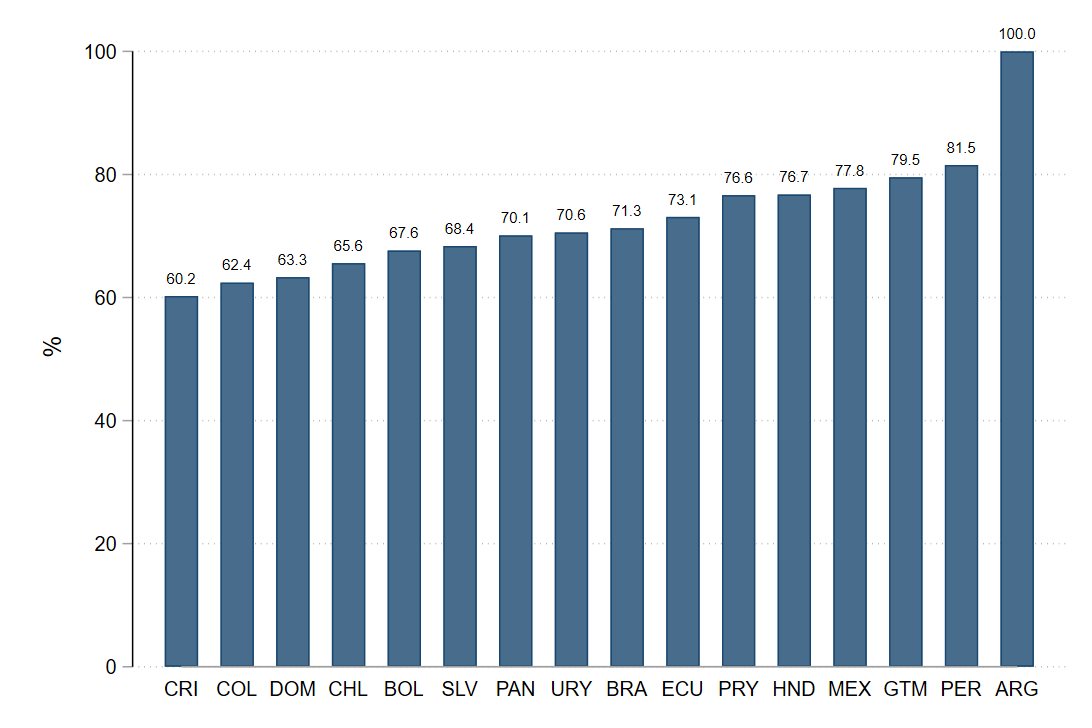
\includegraphics[scale=.3]{latex/figures/Self-employed/se_en_hogar_con_dos_o_mas.png}}
                \label{fig:se-two}
                \footnotesize{Source: SEDLAC}
\end{figure}


\end{document}

